
\chapter{Kauai Experiments 2003}
The Kauai Experiment (KauaiEx) was conducted from June 22 to July 9,
2003 to study high-frequency acoustic propagation for the frequency
range of 8-50 kHz in a shallow water waveguide. In contrast to much
of the previous literature, emphasis was placed on multipath arising
from multiple boundary interactions. The main theme of this
experiment was the role of the environmental physical parameters on
high-frequency acoustic signals applicable to underwater
communications. A great deal of effort was made to characterize the
environment including the surface wave spectrum, 2-D temperature
structure along the propagation path, salinity, currents, and bottom
properties. Using autonomous instruments, most of these parameters
were measured continuously over the two weeks of the experiment
providing information on the ocean volume and surface variability.
At the same time, extensive acoustic measurements were made using a
variety of vertical line arrays some of which spanned the entire
water column. During the course of the experiment there were three
different deployments of acoustic source and receiver arrays. While
a brief overview of the experiment has been provided before [1],
here a description of the experiment during July 01 through July 03
will be discussed.
\begin{figure}[htb]
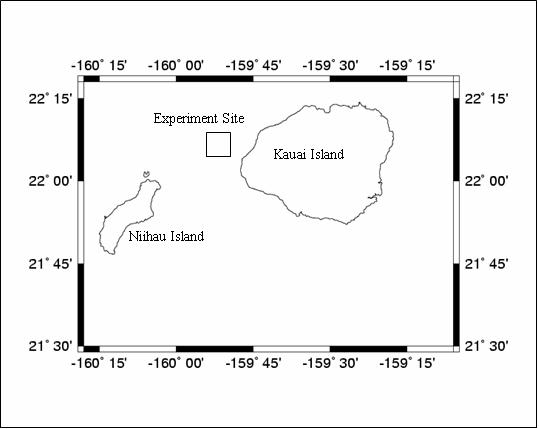
\includegraphics[width=4in]{experimentsite.JPG}
\caption{\normalsize  Map of Kauai Island showing the location of
High Frequency Acoustic Experiment in 2003
}\label{fig-experimentsite}
\end{figure}
\section{Oceanographic Measurements}
Detailed oceanographic measurements made during the experiment
included directional surface waves and water column temperature plus
salinity profiles at different points along a 6-km propagation path.
The current profile, wind speed and direction were also measured at
single points. Figure 1 shows the schematic diagram of the acoustic
and the environmental measurement arrays during the second
deployment. The sea surface waves and temperature profile near the
bottom mounted receiver array for a period of 48 hours (from 11:00
AM July 1 through 10:00 AM July 3, 2003 in GMT time) are presented
here. During this time the temporal variability of acoustic signals
is shown to be correlated with the environmental variability.

%\subsection{Wind}
\subsection{Temperature}
Five thermistor arrays were placed along the propagation track to
measure temporal and spatial distribution of the sound speed during
the experiment. Measurements of the salinity profile at different
points showed a negligible variation. Therefore, here the salinity
is considered constant for calculation of the sound speed profile.
For data discussed here, the temperature profile (UDEL Themistor
String in Fig. 1) near the receiver array at 2 km from the sound
source is shown in Fig. 2. This time corresponds to the same period
for which both surface waves and the acoustic propagation
measurements were made. It is noticed that for most of this time the
water column is a very well mixed layer down to about 50 m depth. A
cold layer (about 4-5 degrees C lower than the mixed layer) emerges
at nearly tidal cycles. Variations of this layer pertaining to
oceanographic features are repeated during the entire experiment.
\begin{figure}[htb]
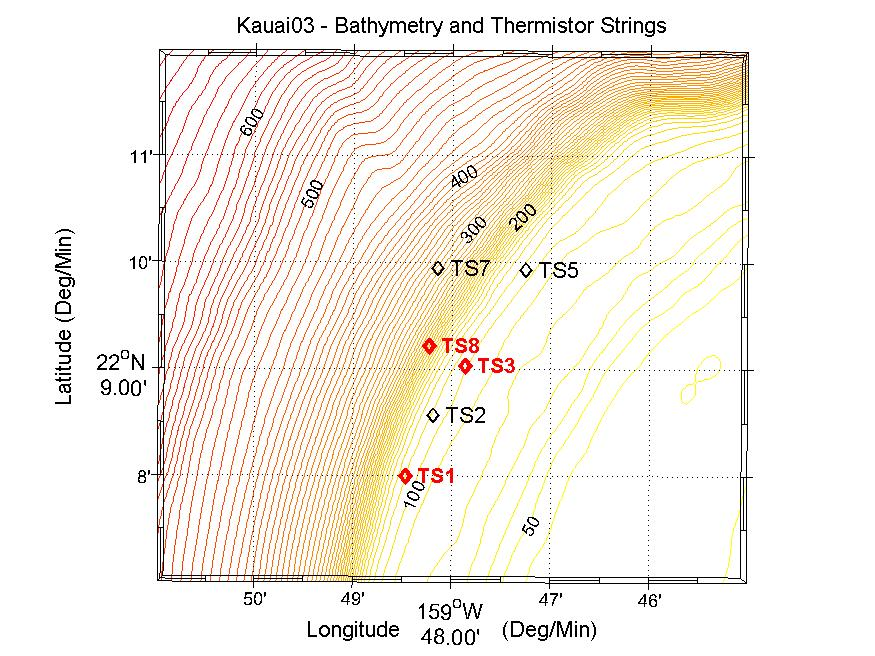
\includegraphics[width=4in]{thermistorsPositions.jpg}
\caption{\normalsize  Location of the thermistor strings moored for
the experiment. Mooring number 1, 2, 3, and 5 have been moored along
the 100m isobath, while mooring number 7 and 8 sample deeper waters
above the slope. }\label{fig-thermistors}
\end{figure}
\subsection{Wind and Surface Wave}
Hourly measurements of wave frequency spectra were made during the
entire experiment using a directional buoy. The wave spectrum and
the wind speed for the period from 11:00 AM July 1 through 10:00 AM
July 3, 2003 are shown in Fig. 3. The right plot shows hourly
measurements of the non-directional wave frequency spectra.  These
plots show that changes in spectral level correspond to changes in
wind speed.   Changes in high-frequency spectral levels are abrupt
while changes in low frequency spectral levels occur gradually. It
is noticed that surface wave energy changes in three different
distinct frequency bands. Open ocean swells show up on (0.05 - 0.1
Hz) which are low frequency waves traveling in from the open ocean
from far distances. Then the wind generated surface waves arrive at
two different bands. First, there are larger scale waves formed
after the wind has blown in the same direction for some duration of
time (0.1 -0.2 Hz), and then small scale surface chop (0.2-0.35 Hz)
that appears almost immediately after wind speed increases and
disappears shortly after wind speed decreases or changes direction
(this is referred to as the land breeze effect). Changes in spectral
levels for the 0.2 - 0.3 Hz small scale, surface-chop frequency show
an immediate increase and decrease corresponding to changes in wind
speed.  Spectral levels for the 0.1 - 0.2 Hz larger scale
wind-generated waves show the same correspondence to changes in wind
speed, but spectral level changes occur on longer time scales.
Energy remains in this frequency band for sometime after wind speeds
decrease.

For both days covered in this period, wind speeds undergo a late
morning increase and a late night decrease.  Changes in spectral
levels for the 0.2 - 0.3 Hz small scale, surface-chop frequency show
an immediate increase and decrease corresponding to changes in wind
speed.  Spectral levels for the 0.1 - 0.2 Hz larger-scale wind
generated waves show the same correspondence to changes in wind
speed, but spectral level changes occur on longer time scales.
Energy remains in this frequency band for some time after wind
speeds decrease and generally the dominant wave direction
corresponds to wind direction. This indicates the majority surface
wave energy is coming from wind-generated waves.

In an acoustic measurement the sea-surface fluctuations may induce
fast fluctuations in the acoustic signal propagation while temporal
variability of the sound speed profile may induce large-scale
fluctuations. To resolve both these scales, we consider different
sampling of the ocean on both short and long geophysical time
scales.

\subsection{Current}
\section{Acoustic Measurements}
\subsection{Transducer}
The Telesonar Testbeds, developed at SPAWARSYSCEN San Diego and
funded by ONR, played a central role in the experiment by providing
two sound sources and two receivers.  These unique, high-fidelity,
modular, reconfigurable, autonomous, wideband instruments were
designed for high-frequency acoustic propagation and communication
research.  Each Testbed is configurable as a transmitter, receiver
or both.  The transmit-configured mooring is 6 meters long and has a
mass of 46 kg in air 19 kg in water.  This extremely small size and
lightweight allow frequent field tests from an array of surface
vessels down to 7 meters in length. The Testbed transmitters are
capable of sourcing arbitrary waveforms at 183 dB in three frequency
bands, i.e. 8-16, 14-22, 25-50 kHz. The receiver-configured Testbeds
are instrumented with a 4-channel 1.5 - 22 kHz, and a 2 channel
1.5-50 kHz receive arrays.  Inside the electronics canister, a
microcontroller coordinates the mission.  A single-board computer
running a robust real-time operating system under DOS orchestrates
the sourcing and recording of data from and to a hard-disk drive.  A
MFSK modem is incorporated into the instrument to provide a link for
remote control and status.  The microcontroller, robust real-time
operating system, and the modem all combine to ensure reliable
mission execution.

Of a series of high frequency acoustic signals transmitted by the
Telesonar Testbed, the probing LFM signal will be used in the
analysis. The LFM signal swept from 8 kHz to 14 kHz in 50 ms. It is
in the low band specified in KauaiEx, which is the nominal 8-14 kHz
frequency band. The LFM signal repeated every 0.25 s for about 60 s.
The LFM signals were transmitted every half hour throughout the
second deployment.
\subsection{Receiver Arrays}
\subsubsection{APL array}
%In the experiment, the APL array was well placed for the studies of
%the surface wave effects on the acoustic wave propagation. In this
%section, these surface wave effects will be shown in both the short
%geo-time scale, in seconds, and the long geo-time scale, in hours.
%Fig. A shows the structure of the Green's function, as known as
%channel impulse response function, obtained from received LFM
%signals. The LFM signal has 50 ms duration, sweeping 8 kHz to 16
%kHz. Every 250 ms, the LFM signal was repeatedly transmitted for 60
%s and received on the APL array about the first 20 s. The LFM
%transmission repeated on every half hour from 21:00 July 1, (GMT) to
%15:00 July 2, 2003. To obtain a better resolution, incoherent
%average of channel impulse response function over 17 seconds is
%shown. By the ray trace and arrival times in Figs. 5 and 6, it is
%concluded that the first peak corresponds to the direct path. The
%second peak is the first bottom path. The third is the first surface
%path. The fourth is the bottom-surface path, as shown in the figure.
%The later arrivals are the multiple bounce paths. In the following,
%only the first four paths are examined in detail. For the direct
%path and the first bottom path, the arrival time and intensity are
%affected by the movement of the APL array, in the short geo-time
%scale, and the change in the water column, in the long geo-time
%scale. The two surface paths are the result of the reflection from
%the dynamic sea surface. Therefore, in addition to those parameters
%affecting the first two paths, the surface wave effects should be
%shown in the propagation property of these surface paths. Fig. B
%shows the channel impulse response function in 17-second duration
%under different surface wave conditions. The channel under a rough
%surface condition is shown on the upper plot. The lower plot shows
%the channel at a relatively calm surface condition. Strength and
%coherence of the surface bounces, corresponding to arrival time
%between 5 ms and 10 ms, in these two plots show distinct differences
%during the 17-second period. At the calm sea condition, the surface
%paths contain much high energy.
For the measurements considered in this paper, the University of
Washington Applied Physics Laboratory autonomous receiving array was
positioned 1.0 km downrange from the bottom-mounted transmitter. A
railcar wheel served as anchor for the array while a 94 cm float at
depth 10 m and several smaller shallow floats kept it approximately
vertical.   The array had eight hydrophones with 2.00 m spacing, the
shallowest at nominal depth 22 m. Each hydrophone (International
Transducer Corporation model 6050C) had an approximately spherical
directivity pattern.  The received waveforms on each hydrophone were
sampled at 50 kHz for a total data throughput of 400 kilosamples/s.
The main processing electronics were contained in a subsurface
canister at nominal depth 12.5 m.  The system could record 40 s
segments before writing the digitized signals to the hard drive.  A
floating radio modem permitted communication with the array and was
used to set the recording schedule, assess the data quality, and
adjust the amplifier gains.  A floating battery pack provided power
and could be replaced without recovering the entire array.  The
array was recovered at the end of the two-week experiment by
signaling a Benthos acoustic release positioned directly above the
anchor. The recording time of the APL array was from 21:00 on July
01 to 15:00 on July 02, 2003
\subsubsection{MPL array}
The Marine Physical Laboratory (MPL) autonomous receiving array was
at 3 km range from the Tested transmitter. The 16-element MPL array
spanned the entire water column from 20 m to 95 m water depth and
the received waveforms on each hydrophone also were sampled at 50
kHz.

The recording time of the MPL array was from 04:00 on July 02 to
07:00 on July 03, 2003. Recorded acoustic data for these three
arrays is labeled APL, UD, and MPL in Fig. EXP-x. The overlapping
period when all three arrays recorded the same signals and were
subjected to the same environmental variability was from 4:00 to
15:00 on July 02, 2003.

\subsubsection{UDel arrays}
During the second deployment mentioned above, the University of
Delaware autonomous receiving array was deployed at 2.0 km from the
Testbed transmitter and about 1.0 km downrange from the APL array.
This array also had eight hydrophones spaced about 0.6 m with the
bottom hydrophone about 0.5 m above the sea floor. The sampling rate
of the UD array was 48 kHz for a total throughput of xx
kilosamples/s. The array response has about 15 dB dynamic range. The
array was mounted inside a rigid tripod to prevent any lateral
motion due to the currents and it has 48 hours of continuous
measurement capability. The recording time of the APL array was from
22:00 on July 01 to 06:00 on July 02, 2003.

% The 8-hydrophone
%receiver array mounted in a vertical stave has roughly a 4 m
%aperture. This array is used in a beamforming algorithm designed to
%provide better resolution of the ray arrivals by showing the
%acoustic field arrival in both time and angle.
